% 4022 Project Thesis Template
% University of Cape Town Department of Electrical Engineering
% Template Version 0.1 - August 2021
% Adapted from the following 2 sources by J Wyngaard
% https://code.engineering.queensu.ca/ece/thesis-template-for-latex
% https://github.com/jpt13653903/LaTeX_UCT_Report.git

% NOTES TO USER:
% You should not need to edit this file (aside from section "TITLE PAGE"). Edit the individual files that are loaded. 
% For example, where you see \phantomsection
\prefacesection{Abstract}

% INSERT YOUR ABSTRACT %
In this work we describe a novel Thesis Template, to be used by students in Electrical \& Engineering at the University of Cape Town. This section entails the abstract of the document. 

%--------------------------------------------------------------------
% Taken from "Scientific Writing by D. Branch Moody"
%--------------------------------------------------------------------
% The abstract is 2 to 6 sentences long and is always less than 500 
% words.  Abstracts are increasingly less than 200 words, 
% according to journal rules. The abstract outlines three points: 
% the field's gap in knowledge, the outcomes of experiments and their
% impact on the field. 
%
% In learning to write abstracts for national meetings, you were 
% probably taught to include descriptions of individual experiments 
% and methods.  The "national meeting" abstract is your only 
% chance to communicate results to the reviewers, so is longer 
% and more detailed.
%
% The abstract submitted to a journal for publication is 
% immediately followed by all of the experiments, so the abstract 
% itself does not need to list every finding and method.  Thus, an  
% abstract for a paper submitted to a journal is usually more 
% conceptual and clearly states the take home point. Increasingly,
% journals have shortened the allowed length of abstracts with 
% many now in the range of 100 to 200 words. Journals now strongly
% encourage authors to focus on the conceptual advance rather 
% than the serial of listing individual experiments. Readers are
% usually interested in why the work is new and important and 
% not a detailed listing of the mouse strains and monoclonal
% antibodies used. 
%
% 'Current knowledge ends' statement. Experienced writers are 
% careful to say where knowledge ends in a statement that comes 
% before the explanation of the new data starts.  The "current 
% knowledge ends" statement, if well crafted, will make it self 
% evident how the new data in the submitted is original or important.
% For example, the second sentence of an abstract could say 
% "Current knowledge of human CD1-reactive T cells derives mainly 
% from study of individual T cell clones, but the roles of such 
% T cell in vivo are not known."  This creates the general 
% expectation that the data that follow are opening up new avenues, 
% yet still allows the reader to decide if the point is proven. 
%--------------------------------------------------------------------, this loads your abstract from the file at Thesis/3_Preface/0_Preface/0_Abstract.tex. Open the file 0_Abstract.tex and edit.

% -> FILE DESCRIPTION :: Thesis.tex
%	This is the master file for your write-up.  It will combine all of the files together to create your thesis (Thesis.pdf). 

%	Thesis.tex will perform the following actions:
%	 1) Import all the supplemental packages
%	 2) Set the styling for the document
%	 3) Combine the various chapters, sections and other components of your thesis into one document.
%	 4) Create LaTex generated sections, such as Table of Context, Glossary, and Bibliography  

%*************************************************************************************************************
% DO NOT MODIFY:
%*************************************************************************************************************

% 4022 Project Thesis Template
% University of Cape Town Department of Electrical Engineering
% Template Version 0.1 - August 2021
% Adapted from the following 2 sources by J Wyngaard
% https://code.engineering.queensu.ca/ece/thesis-template-for-latex
% https://github.com/jpt13653903/LaTeX_UCT_Report.git

% -> FILE DESCRIPTION :: Preamble.tex
%	This files defines the imports necessary for proper compiling of the thesis document and create the styling of the document.

%*************************************************************************************************************
% DOCUMENT
%*************************************************************************************************************
% -> This section defines the basic thesis document. 

% Set Document Type
\documentclass[12pt]{report}  

% Select Thesis Package
\usepackage{0_Config/1_Styles/UCT_EE_Thesis_Style}
    
%*************************************************************************************************************
% PATCHING
%*************************************************************************************************************
% -> This section imports functionality which fixes Latex bugs

\usepackage{morewrites}
%\usepackage{scrwfile}

%*************************************************************************************************************
% SPACING
%*************************************************************************************************************
% -> This section defines the basic spacing options for the thesis document. 

%\usepackage{indentfirst} % Indent first paragraph after header
\setlength{\parindent}{0pt}  % normal paragraph indent
\usepackage{indentfirst}  % ensures first paragraph after section is indented
\setlength{\parskip}{1em}  % vertical space between paragraphs

%*******************************************************************************
% HEADINGS
%*******************************************************************************
% -> This changes the headings go that they are prettier, this can be commented out for traditional headings.

\usepackage{sectsty}

%*************************************************************************************************************
% FONTS
%*************************************************************************************************************
% -> This section defines the fonts for various document entities.

\allsectionsfont{\bfseries}% set all the section font to bfseries
\chapterfont{\Huge} % set the sizes of chapters, sections ...
\sectionfont{\Large}
\subsectionfont{\large}

%*************************************************************************************************************
% FORMATTING
%*************************************************************************************************************
% -> This section defines formatting Table of Contents entr
% example: Chapter 1 Introduction

\usepackage[subfigure]{tocloft}
\usepackage{tocloft}
\usepackage{multicol}

\renewcommand{\cftchappresnum}{Chapter }
\renewcommand{\cftchapaftersnum}{:}
\renewcommand{\cftchapnumwidth}{7em}

% for formatting Table of Contents entry for Appendix, example: Appendix 1: Stuff
\newcommand*\updatechaptername{%
   \addtocontents{toc}{\protect\renewcommand*\protect\cftchappresnum{Appendix }}
}

%*******************************************************************************
% FOOTNOTES
%*******************************************************************************
% -> This section defines formating for footnotes

\interfootnotelinepenalty=10000 % This line stops footnotes from splitting onto two pages.

%*******************************************************************************
% VERBATIM
%*******************************************************************************
% -> 

\usepackage{moreverb}        % Using this package to get better control of the
                             % verbatim environment, mostly for the use of the
                             % listing environment which puts line number
                             % beside each line.  Note that there has to be a number
                             % in each set of brackets, i.e., \begin{listing}[1]{1}.
                             % PDF info file is "The moreverb package" by
                             % Robin Fairbairns (rf@cl.cam.ac.uk) after
                             % Angus Duggan, Rainer Schopf and Victor Eijkhout, 2000/06/29.
%-------------------------------------------------------------------------------
%\usepackage{verbatim}        % allows the use of \begin{comment} and \end{comment}
                             % as well as \verbatiminput{file}
                             % Note:  when using verbatim to input from a text file,
                             % such as a specification or code, use \begin{singlespacing}
                             % and \end{singlespacing}.  Also, tabs are not read
                             % properly, so the input file must only use spaces.

%                             \begin{comment}
%                             Can also use the verbatim package for
%                             comments like this...
%                             \end{comment}


%*******************************************************************************
% GLOSSARY
%*******************************************************************************
% -> Creates the glossary

\usepackage[acronym,automake,toc]{glossaries}
\newglossary[slg]{symbol}{sym}{sdn}{List of Symbols}
\makeglossaries

% See Glossary/Glossary.tex for the content of your glossary

%*******************************************************************************
% INDEX
%*******************************************************************************
% -> Creates the Index

\usepackage{makeidx}         
\makeindex

%*******************************************************************************
% MATH
%*******************************************************************************
% -> Import and configure packages for math
\usepackage{mathrsfs}		 % For Symbols
\usepackage{amssymb}		 % For More Symbols
\usepackage{amsfonts}		 % For Other Symbols
\usepackage{amsmath}         % For Equations
\usepackage{amsthm}          % For Theorems & Definitions


% Using the amsthm package, define a new theorem environment for my
% definition.  * means don't number it.
\newtheorem*{definition}{Definition}
\usepackage{cases}           % to make numbered cases (equations)
\usepackage{calc}            % Used with the Ventry environment defined below.

%*******************************************************************************
% FLOATS, PLOTS, AND FIGURES
%*******************************************************************************
% -> This section defines and configures packages for various styles of floating objects and figures. 
 
\usepackage{graphicx}       % for graphic images (use \includegraphics[...]{file.eps})
%\usepackage{subfigure}      % for subfigures (figures within figures)
\usepackage{subfig}			% for subfigures (figures within figures). Same as subfigures except it works.
\usepackage{wrapfig}		% for wrapping text around figures
%\usepackage{boxedminipage}  % to make boxed minipages, i.e., boxes around figures
\usepackage{rotate}         % for use of \begin{sideways} and \end{sideways}
\usepackage{listings}       % for use of printing code blocks
\usepackage{pgfplots}		% for plots
\usepackage{pdfpages}		% for importing PDFs
\usepackage{geometry}

% Define how the ``listings'' to look.
%\lstset{basicstyle=\footnotesize,, numbers=left, numberstyle=\small, stepnumber=1, numbersep=5pt, showspaces=false, lineskip=-1pt}

\usepackage{float}           % Using this package to get better control of floats
                             % including the ability to define new float types for
                             % specification and code listings.
                             % DVI info file is "An Improved Environment for Floats"
                             % by Anselm Lingnau, lingnau@tm.informatik.uni=frankfurt.de
                             % 1995/03/29.

% Style of float used for code listings
\floatstyle{ruled}
\newfloat{Listing}{H}{lis}[chapter]
\renewcommand{\lstlistlistingname}{List of Code Listings} % Title be changed as necessary

                             % Note:  The listings don't have space between the chapters, unlike
                             % the standard list of tables etc.  At the end, copy the spacing
                             % commands from the .toc file and insert into the .lis file.  Then,
                             % DO NOT LATEX it again, simply go to the DVI viewer!

\usepackage{placeins} % for \FloatBarrier which stops floats from crossing a point

%*******************************************************************************
% TABLES
%*******************************************************************************
% -> This section defines tables

\usepackage{tabularx}        % Package used to make variable width-columns, i.e.,
                             % column widths are changed to fit the maximum width
                             % and text is wrapped nicely.

\usepackage{threeparttable}

\usepackage{lscape}			% For landscape
\usepackage{adjustbox}		% To adjust table width
\usepackage{multirow}		% For merging and splitting table cells

%*******************************************************************************
% CAPTIONS
%*******************************************************************************
% ->  This section defines captions

\usepackage{caption}   % Package used to make my captions 'hang', i.e., wrap around, but not under the name of the caption.
%\usepackage[justification=centering]{caption} % Captions that are centered
                             

% Find that the captions are too far from my verbatim figures, but if
% I change it to 0, then the captions are too close for my other types
% of figures.  Maybe set each one separately?
%\setlength{\abovecaptionskip}{1ex}

%\setlength{\textfloatsep}{1ex plus1pt minus1pt}

%\setlength{\intextsep}{1ex plus1pt minus1pt}

%\setlength{\floatsep}{1ex plus1pt minus1pt}

%*******************************************************************************
% MISCELLANEOUS
%*******************************************************************************
% ->  This section defines miscellaneous packages that facilitate miscelaneous things

\usepackage{layout}          % useful for determining the margins of a document
                             % use with \layout command
                             
\usepackage{changebar}       % Way of indicating modifications by putting bars in the
                             % margin.  Read about it in "The Latex Companion".
                             
\usepackage{enumitem}		% For enumerated lists


\usepackage{siunitx}        % Used for typesetting units

%*******************************************************************************
% REFERENCES ETC.
%*******************************************************************************
% ->  This section defines the reference section

\usepackage{varioref}        % Better page references, e.g., "on preceding page", etc.
                             % \vref{key} Create an enhanced reference.
                             % \vpageref[text]{key} Create an enhanced page reference.
                             % \vrefrange{key}{key} Create an enhanced range of references.
                             % \vpagerefrange[text]{key}{key} Create an enhanced range of page references.
                             % Note: doesn't really work for consecutive pages.

% Renewing the text for before and after
\renewcommand{\reftextafter}{on the next page}
\renewcommand{\reftextbefore}{on the previous page}
\usepackage{url}             % for use of \url - pretty web addresses
\usepackage{fancyhdr}
\usepackage{cite}
\usepackage{notoccite}      % Prevents references from starting in TOC, List of Figures, etc.

%*******************************************************************************
% Block Diagrams
%*******************************************************************************
% ->  This section defines imports for block diagrams and flow charts

\usepackage{tikz}
\usetikzlibrary{arrows,automata,arrows.meta}

% Block Diagram
\tikzstyle{block} = [draw,fill=blue!20,minimum size=2em]
\def\radius{.7mm} 
\tikzstyle{branch}=[fill,shape=circle,minimum size=3pt,inner sep=0pt]

% Flow Charts
\usepackage{pgf}
\usepackage[utf8x]{inputenc}
\usetikzlibrary{positioning,calc}
\tikzset{
	state/.style={
		rectangle,
		rounded corners,
		draw=black, very thick,
		minimum height=2em,
		inner sep=2pt,
		text centered,
	},
}

%*******************************************************************************
% HYPERLINKS (must be last)
%*******************************************************************************
% ->  This section defines how hyperlinks function

% Uncomment these next two lines for linkback to citation pages in biblio
%%#\renewcommand*\backref[1]{\ifx#1\relax \else \linebreak Cited on page(s): #1. \fi}

\hypersetup{
	colorlinks=true,  % Change links to being coloured text, no boxes
	linkcolor=blue,
	urlcolor=blue,
    citecolor=blue
}
% Neat package to turn href, ref, cite, gloss entries
% into hyperlinks in the dvi file.
% Make sure this is the last package loaded.
% Use with dvips option to get hyperlinks to work in ps and pdf
% files.  Unfortunately, then they don't work in the dvi file!
% Use without the dvips option to get the links to work in the dvi file.

% Note:  \floatstyle{ruled} don't work properly; so change to plain.
% Not as pretty, but functional...
% The bookmarks option sets up proper bookmarks in the pdf file :)

% Need this command to allow hyperref to play nicely with gloss; otherwise
% almost every \gloss will cause an error...
%%#\renewcommand{\glosslinkborder}{0 0 0}

\usepackage[colorinlistoftodos]{todonotes}
\newcommand{\todoall}[1][]{\todo[color=yellow, inline]}
\begin{document}

%*************************************************************************************************************
% TITLE PAGE 
%	INSERT THE DETAILS OF YOUR THESIS
%	REMOVE THE '%' TO UN-COMMENT LINE
%*************************************************************************************************************
\makeatletter
\title{Digitised ECG Mobile App}\let\Title\@title
\author{Dimpho Sefora}            \let\Author\@author
\makeatother

\supervisor{Dr. Yaaseen Martin}
\dept{Electrical Engineering}
\degree{Electrical and Computer Engineering}
\copyrightyear{2021}

\beforepreface

%*******************************************************************************
% ABSTRACT
%*******************************************************************************
\phantomsection
\prefacesection{Abstract}

% INSERT YOUR ABSTRACT %
In this work we describe a novel Thesis Template, to be used by students in Electrical \& Engineering at the University of Cape Town. This section entails the abstract of the document. 

%--------------------------------------------------------------------
% Taken from "Scientific Writing by D. Branch Moody"
%--------------------------------------------------------------------
% The abstract is 2 to 6 sentences long and is always less than 500 
% words.  Abstracts are increasingly less than 200 words, 
% according to journal rules. The abstract outlines three points: 
% the field's gap in knowledge, the outcomes of experiments and their
% impact on the field. 
%
% In learning to write abstracts for national meetings, you were 
% probably taught to include descriptions of individual experiments 
% and methods.  The "national meeting" abstract is your only 
% chance to communicate results to the reviewers, so is longer 
% and more detailed.
%
% The abstract submitted to a journal for publication is 
% immediately followed by all of the experiments, so the abstract 
% itself does not need to list every finding and method.  Thus, an  
% abstract for a paper submitted to a journal is usually more 
% conceptual and clearly states the take home point. Increasingly,
% journals have shortened the allowed length of abstracts with 
% many now in the range of 100 to 200 words. Journals now strongly
% encourage authors to focus on the conceptual advance rather 
% than the serial of listing individual experiments. Readers are
% usually interested in why the work is new and important and 
% not a detailed listing of the mouse strains and monoclonal
% antibodies used. 
%
% 'Current knowledge ends' statement. Experienced writers are 
% careful to say where knowledge ends in a statement that comes 
% before the explanation of the new data starts.  The "current 
% knowledge ends" statement, if well crafted, will make it self 
% evident how the new data in the submitted is original or important.
% For example, the second sentence of an abstract could say 
% "Current knowledge of human CD1-reactive T cells derives mainly 
% from study of individual T cell clones, but the roles of such 
% T cell in vivo are not known."  This creates the general 
% expectation that the data that follow are opening up new avenues, 
% yet still allows the reader to decide if the point is proven. 
%--------------------------------------------------------------------   

%*******************************************************************************
% ACKNOWLEDGEMENTS
%*******************************************************************************
\phantomsection
\prefacesection{Acknowledgments}

% INSERT YOUR ACKNOWLEDGEMENTS %
%I would like to acknowledge my parents and friends. This thesis, a manifestation of the many sleepless nights, would not have been possible without their support. This section highlights your acknowledgment of individuals whom you believe deserve recognition for their contribution towards making your achievement possible.  

\clearpage % keep this for proper page numbering!   

%*******************************************************************************
% PLAGIARISM DECLARATION
%*******************************************************************************
\phantomsection
\prefacesection{Plagiarism Declaration}

    \begin{enumerate}
        \item I know that plagiarism is wrong. Plagiarism is to use another's work and pretend that it is one's own.
        \item I have the IEEE convention for citation and referencing. Each contribution to, and quotation in, this final year project report from the work(s) of other people, has been attributed and has been cited and referenced.
        \item This final year project report is my own work.
        \item I have not allowed, and will not allow, anyone to copy my work with the intention of passing it off as there own work or part thereof.
    \end{enumerate}

    \vspace{15mm}
    \begin{figure}[h]
        \hspace{10cm}
\includegraphics[width=0.2\linewidth]{2_Preface/DS-signature.jpg}
    \end{figure}
    \mbox{}\hfill\begin{minipage}{65mm} % No need to change this part
      \dotfill\\[1ex]%
      \Author\\
      \today
    \end{minipage}
    
    \vfill\vfill\vfill

   

%*******************************************************************************
% Table of Contents
%*******************************************************************************
% Print the Table of Contents 
\PageContentstrue

% To disable, use the following:
%\PageContentsfalse

%*******************************************************************************
% The following lists can be commented out if not necessary for your thesis:
%*******************************************************************************

%*******************************************************************************
% Glossary
%*******************************************************************************
% The Glossary 
\PageGlossariestrue

% To disable, use the following:
%\PageGlossariesfalse

% Include Glossary
% -> FILE DESCRIPTION :: Glossary.tex
%	This files contains all of your glossaries. It has been configured to have your main glossary (definitions), acronym glossary and symbols glossary.

% ---------------------------------------------------------------------------------------------%

% MAIN (Definitions) GLOSSARY
% \newglossaryentry{NameInLink}{
%	name={NameToShow},
%	sort=NameInSort,
%	description={What does it mean?}
%	}

\newglossaryentry{diction}
{
	name={diction},
	sort=diction,
	description={the choice and use of words and phrases in speech or writing}
}
\newglossaryentry{lexicon}
{
	name={lexicon},
	sort=lexicon,
	description={the vocabulary of a person, language, or branch of knowledge}
}

\newglossaryentry{prose}
{
	name={prose},
	sort=prose,
	description={written or spoken language in its ordinary form, without metrical structure}
}
\newglossaryentry{ADC}
{
	name={ADC},
	sort=ADC,
	description={Analogue-to-Digital Converter}
}

\newglossaryentry{ECG}
{
	name={ECG},
	sort=ECG,
	description={Electrocardiogram}
}

\newglossaryentry{depolarization wave}{
	name={depolarization wave},
	sort=depolarization wave,
	description={the wave of electrical activity that spreads through the heart muscle, causing it to contract}
}

% ---------------------------------------------------------------------------------------------%

% ACRONYMS
% \newacronym{NameInSort}{NameToShow}{Definition}
\newacronym{lol}{LOL!}{Laugh Out Loud}


% ---------------------------------------------------------------------------------------------%

% SYMBOLS
% \newglossaryentry{NameInLink}{
%	type=symbol, 
%	name={NameToShow},
%	sort=NameInSort,
%	description={What does it mean?}
%	}

\newglossaryentry{mySymbol}{
	type=symbol,
	name={\textrm{$\Upsilon$}},
	sort=thresh,
	description={Arbitrary symbol.}
}



% This line forces all entries into glossary, even if they have not been referenced
% UNCOMMENT THIS LINE TO INCLUDE ALL GLOSSARY ITEMS (Not just those referenced)
% \glsaddall

% UNCOMMENT INDIVIDUAL GLOSSARIES TO BE PRINTED (IF not using \PageGlossariestrue) %
% \printglossaries % Prints ALL glossaries.
% \printglossary % Print the terms glossary
% \printglossary[title = Nomenclature] % Print the terms glossary
% \printglossary[type=symbol, title=List of Symbols] % Prints the acronym glossary
%\printglossary[type=\acronymtype,title=Glossary of Abbreviations] % Prints the abbreviation glossary

%*******************************************************************************
% List of Tables
%*******************************************************************************
% Print the List of Tables
\PageTablestrue

% To disable, use the following:
%\PageTablesfalse

%*******************************************************************************
% List of Figures
%*******************************************************************************
% Print the List of Figures
\PageFigurestrue

% To disable, use the following:
%\PageFiguresfalse


%*******************************************************************************
% List of Code Snippets
%*******************************************************************************
% Print the List of Code Snippets
%\PageCodeSnippetstrue

% To disable, use the following:
\PageCodeSnippetsfalse

%*******************************************************************************
% List of Equations
%*******************************************************************************
% Print a list of all equations
%\PageEquationstrue

% To disable, use the following:
\PageEquationsfalse

%*******************************************************************************
% Apply Apply After Preface - DO NOT MODIFY
%*******************************************************************************
% Create afterpreface sections
\afterpreface


%*******************************************************************************
% 0.7 - CHAPTERS
%*******************************************************************************
% Include Chapters. Chapters are kept separated to make editing easier.

% Chapter 1 - Introduction

\glsresetall % reset the glossary to expand acronyms again
\chapter[Introduction]{Introduction}\label{ch:Introduction}
\index{Introduction}

Electrocardiograms are one of the first tests conducted when one is admitted to the hospital. They provide a wealth of information on the health of a patient. However, they continue to be produced in paper format. This means they must be stored for longevity in large storage rooms

\section{Background}
% Should there be a motivation? A quote? 
An electrocardiogram \gls{ECG} is a technology that both measures and records the electrical signal patterns describing the rhythmic activity of the heart. These electrical pulses are what signal the heart's skeletal muscles to undergo ventricular contraction \cite{AlGhatrif2012}. Irregularities from the expected patterns provide a wealth of information on the patient's condition.

Clinically, two ECG systems are in use: paper-recorded and computer-based. Paper ECGs remain the foundational format and are routinely requested as an initial diagnostic test \cite{AlGhatrif2012}. Computer-based ECGs, first introduced in the 1960s \cite{Medved2020CriticalAO}, aimed to reduce the dependency on specialist interpretation, but continue to face issues of diagnostic reliability and digital record management \cite{Heaney2022InternetOT}. Furthermore, due to significant technological and logistic barriers associated with accessibility and cost, the widespread adoption of these systems has been limited \cite{Rubbo2015UseOE}\cite{Qiu2023AutomatedCR}. Therefore, paper ECGs remain widely produced. However, their physical form presents a persistent limitation: secure and accessible storage for later interpretation. Addressing this challenge motivates the digitisation of paper ECGs into formats that can be efficiently stored and accessed, especially for the long-term treatment of cardiac patients \cite{Ravichandran2013NovelTF}.

Manual digitisation, which involves manually scanning or transcribing paper ECG tracings into digital systems, is a popular solution to this issue.  Although this technique eventually makes it possible to save ECGs in electronically, it is expensive, time-consuming, and prone to errors, especially in environments with lots of patients \cite{Eapen2016MobileHealthCardioEHR}. % These drawbacks significantly limit its practicality as a long-term solution

Recent developments in mobile health technologies suggest a potential pathway to address this limitation. Smartphones, with their widespread availability and camera facilities, enable paper ECGs to be captured, digitised, and stored within mobile applications \cite{MartinezPerez2013MobileAppsCardiology}\cite{Wu2022FullyAutomatedECGDigitisation}. This strategy creates a way to bridge the gap between affordable availability to digital ECG formats and possibly addressing the storage problem \cite{Liu2020MobileCloudECGExtraction}. Mobile platforms can enhance patient record management and continuity of treatment by enabling the direct archiving and retrieval of ECG information on portable devices. However, while promising, these developments also highlight the need to explore how paper-recorded ECGs can be reliably digitised and integrated into mobile-accessible formats.


\section{Problem Statement}

The digitisation of paper-based electrocardiograms continues to present a challenge, as reliance on physical records causes inefficiencies in storage, retrieval, and long-term accessibility \cite{MartinezPerez2013MobileAppsCardiology,Steinhubl2013CanMHealth}. Despite being widespread, manual digitisation is expensive, inefficient, and prone to errors \cite{Eapen2016MobileHealthCardioEHR} and existing mobile scanning tools are not designed for ECG waveforms, leading to distortion, misalignment, and loss of signal fidelity \cite{McConnell2018CardioMHealthReview}. Current methods are inadequate for efficiently converting paper ECGs into accurate, analysis-ready digital formats, highlighting the need for reliable, mobile-accessible digitisation solutions.


\section{Objectives}
These objectives guide the progression of the research, ensuring that the work done is centred on the problem statement. The following will be objectives will be explored throughout the report: 
\begin{enumerate}
    \item Review literature on ECG signal structure, interpretation, and digitisation techniques.
    \item Investigate existing image processing and signal processing methods for waveform extraction from photographs.
    \item Design and develop a mobile application (Android or iOS) for accurate ECG strip digitisation.
    \item Implement algorithms for noise reduction, de-warping, filtering, and artifact removal.
    \item Store processed ECG signals in a standardised digital format.
    \item Test and evaluate the accuracy and usability of the developed application.
\end{enumerate}

\section{Scope and Limitations}

\textbf{Scope:}
\begin{itemize}
    \item Mobile application development for Android/iOS.
    \item Image capture, processing, and signal extraction for standard ECG paper strips.
    \item Local storage of digitised ECG in standard digital formats.
\end{itemize}

\textbf{Limitations:}
\begin{itemize}
    \item No integration with electronic health record (EHR) systems in this phase.
    \item Limited dataset for testing.
    \item Optimised for standard-format single-lead or multi-lead strips.
    \item No integration of deep-learning analysis and diagnosis of digitised data 
\end{itemize}

\section{Thesis Outline}
\begin{itemize}
    \item \textbf{Chapter 2}: Literature Review --- ECG basics, digitisation methods, and relevant image/signal processing techniques.
    \item \textbf{Chapter 3}: Methodology and Design --- approach, algorithms, and system architecture.
    \item \textbf{Chapter 4}: Implementation --- development process and app features.
    \item \textbf{Chapter 5}: Results and Discussion --- evaluation and performance.
    \item \textbf{Chapter 6}: Conclusion --- summary of findings and future work.
\end{itemize}

% Chapter 2 - Background

\glsresetall % reset the glossary to expand acronyms again
\chapter[Literature Review]{Literature Review}\label{ch:LitReview}
\index{Literature Review}

%What to expact in this chapter

This chapter provides a comprehensive evaluation of literature relevant to the research topic. It begins with an introductory section outlining the motivation for the study, focusing on the need to further investigate mobile app development for digitising and storing ECG paper records. A brief overview of the theory behind ECG signal formation follows, providing the foundation for understanding its digitisation. 

The review then adopts a funnel approach: first examining existing methods of ECG record digitisation, then evaluating the potential of mobile applications for this purpose through image capture, and finally considering techniques for extracting ECG waveforms from images. The chapter concludes with a summary of key findings, identifying gaps in current research and setting the stage for the methodology that follows.

%----------------------------------------------------------------------------------------------

\section{Introduction}

The electrocardiogram (ECG) has been a fundamental tool in medicine since 1901 \cite{MartinezPerez2013MobileAppsCardiology}. Over the years, a vast number of ECG paper records have been produced. Consequently, researchers have devised methods to digitise these records in order to ensure long-term preservation, improve accessibility, and facilitate future evaluation and diagnosis. It is therefore important to investigate and assess these methods to understand their respective strengths and limitations.

With the growing use of mobile applications in healthcare \cite{Steinhubl2013CanMHealth}, new opportunities for ECG digitisation have emerged. This enables investigation into whether ECG images captured with mobile devices can be effectively processed for digitisation.

%----------------------------------------------------------------------------------------------

\section{ECG Fundamentals} \label{sec: ECG_Fund}
% the problem with this section is that it doesn't add points to delebarate over - how advantageous or disadvantageous or how the results sway the decsions

Electrocardiogram signals show how the path of the \gls{depolarization wave} - the flow of a group of positive electric charges - moves during each heartbeat \cite{osmosisECGbasics2025}. Hearts have natural pacemakers that initiate electric signals that cause atrial and ventricular contraction \cite{myhealthSAnode2024}. Electrocardiograms are built to sense these natural signals and convert them into useful information that portray the heart's condition.

\subsection{ECG Signal Generation}

The electric activity of the heart is governed by the sinoatrial (SA) and atrioventricular (AV) nodes. The SA node initialises the impulses and the AV node introduces delays to their delivery to co-ordinate between arterial and ventricular contractions for optimum heart functionality \cite{myhealthSAnode2024}.

As the positive charges move through the heart's muscles, their negative resting state changes to a positive active state. This change in charge of the internal muscles affects a change to the external charge surrounding it \cite{osmosisECGbasics2025}. This creates the potential difference measured by the electrocardiogram electrodes. If detected it is noted as a deflection on the ECG waveform. The bigger the potential difference, the larger the deflection \cite{osmosisECGbasics2025}.

(image explaining or showing ECG deflections - so they know what to look for in the actual trace)

\subsection{ECG Waveform Formation}

An ECG signal consists of five deflections that together form the PQRST complex, representing a single heartbeat and the complete cycle of myocardial contraction and relaxation \cite{AlGhatrif2012}.

The P wave reflects atrial depolarisation, initiating atrial contraction. It is typically a low-amplitude, gently sloped deflection due to the slower propagation of the depolarisation wave through atrial myocardial cells \cite{OReilly2023ModelDrivenAO}. The QRS complex corresponds to ventricular depolarisation and the onset of ventricular contraction, with the R wave being the largest positive deflection \cite{Prima2018PolyanilineAN}. The T wave represents ventricular repolarisation, preparing the ventricles for the next cardiac cycle \cite{Prima2018PolyanilineAN}.

\begin{figure}[H]
    \centering
    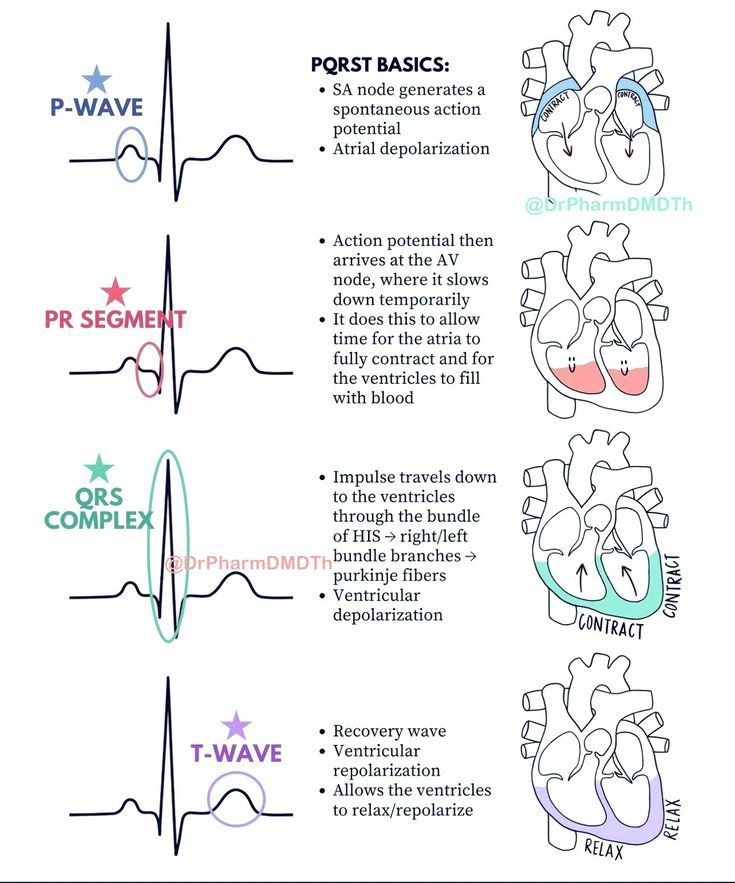
\includegraphics[width=0.4\textwidth]{3_Chapters/2_Chapter_LiteratureReview/Figures/PQRST_complex.jpg}
    \caption{Placeholder for ECG diagram}
    \label{fig:ECG_Waveform}
\end{figure}

The timing and amplitude of the PQRST wave are essential for patient health analysis \cite{Sinha2023SemiSupervisedCD}. Significant signal loss in the digisation process would thus render the ECG useless for diagnostic purposes.

The grid is formed ... such that reading the waveforms can remain consistent throughout.

\subsection{ECG leads}

The direction of this wave is dependent on the leads. The leads are defined by the electrodes used. In a 12-lead ECG, there are 10 electrodes used to measure the heart's activity from different angle and planes. Each lead provides different and vital information about arrhythmias and myocardial infarction (heart attacks). 

There are the limb electrodes places by the left arm and leg and the right arm. Measurements between two of them, with the third being a reference, creates the I, II, and III dipoles leads. When a fourth electrode known as the reference or zero electrode is introduced, the augmented leads are created. This is a measurement from one of the limb electrodes to the reference electrodes. This creates one of the unilateral leads. 

In 1934, it was noted that there were areas in the heart that needed to be measured to better detect myocardial infarctions. This gave birth to the precordial leads through the use of six electrodes placed around the precordial (chest area about and around the heart). 

These make up the 12 leads that illustrate the different waveform patterns seen in the electrocardiogram trace. They are used to section the ECG into 12 important regions which can be segmented and analysed further. \cite{AlGhatrif2012}

%----------------------------------------------------------------------------------------------

\section{Formats for Digitised ECGs}

In recent decades, multiple approaches have been developed for digitising and storing ECG records, ranging from the scanning of paper traces into PDF format to direct digitisation using computer applications such as MATLAB or Python.

\subsection{Scanned PDF Format}

The most straightforward method of digitising ECGs is by scanning paper records into PDF format. This approach makes data easily accessible across multiple devices, such as laptops and mobile phones. It also facilitates better organisation and storage of patient information, improving the efficiency of record retrieval and supporting long-term preservation that physical paper cannot guarantee.

However, this method has notable limitations. Since the ECG remains an image rather than raw signal data, it cannot be manipulated or re-analysed for further processing. Scanned records may contain physical defects such as creases, stains, or fading, particularly when dealing with older paper traces. These issues cannot be corrected during scanning, which reduces the reliability and quality assurance of the data. Thus, while efficient for archiving and accessibility, this approach is limited in its usefulness for future diagnostic and analytical applications.

\subsection{Manual Digitisation}

A more time-consuming approach to ECG digitisation involves manually recording the millivolt–time coordinates of the individual signal leads onto an electronic spreadsheet and entering them into software such as MATLAB or Python. Unlike scanning into PDF format, this method produces a true digital signal that can be manipulated, processed, and analysed with high accuracy. However, it is highly labour-intensive and susceptible to human error, particularly when large volumes of ECG records must be digitised.

\subsection{MATLAB/Python Digitisation}

Technological advancements, along with the development of Python and MATLAB libraries that integrate vision frameworks for object identification, have enabled the efficient extraction of signals from scanned ECG images. Algorithms can now automate the tracing of ECG waveforms into time-series coordinates, which can subsequently be plotted, analysed, and manipulated in digital form. The extracted data are typically stored in CSV format, facilitating efficient organisation, retrieval, and downstream processing.

This approach offers several advantages: automated signal acquisition, reliable digital storage through CSV files, and straightforward visualisation within environments such as MATLAB, Python IDEs, and Excel. Despite these benefits, practical limitations remain. Such tools are generally deployed on laptops or desktop computers, which may not always be accessible in the fast-paced environment of a hospital or outside clinical settings when records are urgently required. Furthermore, most implementations perform best with scanned images and often show reduced reliability when applied to camera-captured inputs, limiting their adaptability in resource-constrained or less controlled settings.

%-------------------------------------------------------

\section{Smartphone-based ECG Capturing}

\subsection{Performance - Resolution (can it handle it)}
%limitations can talk about camera resoluations - development
\subsection{Accessibility and Cost-Effectiveness}

%-------------------------------------------------------

\section{Digitisating ECG Signals}

The fundamental concept of digitising ECG signals lies heavily within image processing. Generally, the process involves preparing the image through filteration and artifact removal, isolating the region of interest, particularly the 12 leads, through segmentation, and converting the extracted ECG waveform into a one-dimensional digital signal suitable. However, machine learning models have also been used to achieve greater results in varying datasets. 

\subsection{Artifact Removal}
%method 1 - which is briefly ... method 2 - briefly ... (add in equations where possible/ table of comparison)
The report written by Cuong et al. highlights how the performance of their model dropped by 60.87\% when artifacts are present in the processed images \cite{Cuong2024}, emphasising the neeed for their removal.

\subsubsection{Shadow and Crease Removal}
%with grayscale ... with RGB (this is where I can add the RBG equation)
Shadows and creases represent the most disruptive artifacts in ECG image digitisation. Mishra et al. intorduces the concept of luminance correction for shadow removal, given that they occur due to obscured light \cite{Mishra2021}. This method involves changing the luminance/brightness of the \gls{ROI} without affecting the colour. This can me done in different colour spaces.

\begin{table}[H]
    \centering
	\caption{Luminance Correction Methods}\label{tab:lumcor}
    \begin{tabular}{|l|>{\raggedright\arraybackslash}p{4cm}|>{\raggedright\arraybackslash}p{3cm}|>{\raggedright\arraybackslash}p{3cm}|l|}
    \hline
    Space        & Description                                        & Strengths                           & Limitations                                       & Cite                 \\ \hline
    RGB          & Adjust luminance in  each channel           & Requires no conversion   & Can erode the colour                                  & \cite{Yang2022LABNetLC}  \\ \hline
    LAB          & Corrects luminance separately from colour   & Luminance and colour well separates & Can introduce noise                        & \cite{Yang2022LABNetLC}  \\ \hline
    YCbCr        & Corrects brightness separately from colour  & Good luminance separation           & Produces less uniform colour               & \cite{Wang2017StackedCG} \\ \hline
    \end{tabular}
\end{table}

\subsubsection{Noise Removal}
%different filters and their pros and cons (make it aplication based)

\textbf{Mean Filters:} Within a pixel cluster of odd nxn sizing, the middle pixel is replaced by the average of all their pixel values. It unfortunately serves to blur the image, removing important object detail \cite{Chauhan2018PerformanceAO}.\\
\textbf{Median Filters:} These are better capable at removing salt and pepper (discrete) noise, while preserving edge details. However, it does tend to remove finer details that appear as outliers in a cluster of pixels \cite{Chauhan2018PerformanceAO}.\\
\textbf{Gaussian Filters:} These better preserve finer details as compared to mean and median filters \cite{Chauhan2018PerformanceAO}. However, they perform poorly when applied to discrete noise.\\
\textbf{Wiener Filters:} In images that have noise caused by motion blur, these filter perform excellently. They are less effective for salt and pepper noise as compared to other linear filters \cite{Chauhan2018PerformanceAO}.

Camera-captured images are littered with continous random noise cause by the hardware involved. This makes filters that tackle Gaussian noise more appealing for the purpose of this project.

\subsubsection{Text Removal}

ECG papers contain labels for each lead. These characters need to be removed before converting the extracted wavform into a 1-D signal.

\textbf{Optical Character Recognition:} Vision frameworks are used to identify text in images. The algorithms than use morphological operators to isolate the regions, and image impairings to reconstruct the area \cite{Ganesh2021CombiningOC}.\\
\textbf{Image Processing:} There are a couple of image processing approaches that can be used to remove text, with most using cropping
\textbf{}

\subsection{Segmentation}
% separating to separate leads (use diagrams I generated in the benchmarking)

\subsubsection{Image Processing Approach}

\subsubsection{Machine Learning Approach}

%after both sections show a comparison table showing the pros and cons of each

\subsection{Background Removal and Signal Extraction}

\subsubsection{Image Processing Approach}

\subsubsection{Machine Learning Approach}

%after both sections show a comparison table showing the pros and cons of each

\subsection{Post-processing}
%Continuity (how it's detected) and what can be done to fix it

\subsection{Signal Digitisation}
%talk about consistency of the approach used, matbe highlight any slight differences in the implementation, use the equation form one of the reports

%-------------------------------------------------------

\section{Conclusion}

\begin{itemize}
    \item Summary of reviewed methods and gaps.
    \item Justification for proposed app.
    \item Key algorithmic challenges for this project.
\end{itemize}

% Literature Review
%\section{Literature Review}
\begin{itemize}
	\item{Broad description of subject}
	\item{Some relevant history}
	\item{Current implementations in industry}
	\item{New \& Related Research on the subject}
\end{itemize}
% Chapter 3 - Methodology
% With Sample Figures From Kevin Hughes

\glsresetall % reset the glossary to expand acronyms again
\chapter[Methodology]{Methodology and Design}\label{ch:Methodology}
\index{Methodology}

This chapter details the design and engineering decisions taken to develop and evantually implement digitising ECG signals through mobile applications. These decisions are guided by the observations highlighted in the \href{ch:LitReview}.

It will begin with a highlevel overview of the proposed approach for tackling the problem. It will then provide specific details on the methods and techniques used in the research, including any algorithms, tools, and technologies employed. The chapter will also discuss the rationale behind these choices, highlighting how they align with the research objectives and address the identified challenges.

%-------------------------------------------------------

\section{Overview of Approach}

The core principle of the proposed approach is iteration. With each new stage of development, earlier steps are revisited to ensure ongoing risk management and continuous improvement. This cyclical process mirrors the spiral model commonly applied in system and software design.

\begin{figure}[H]
    \centering
    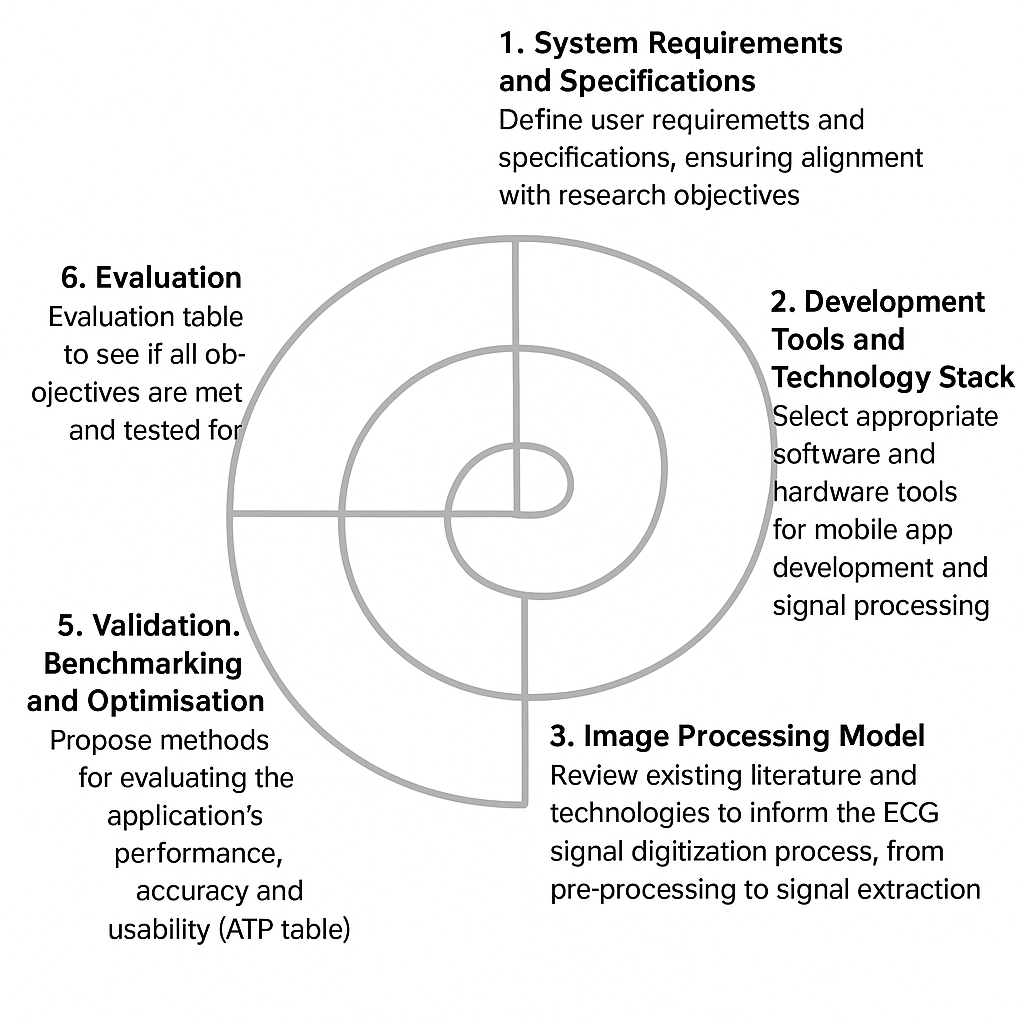
\includegraphics[width=0.7\textwidth]{3_Chapters/3_Chapter_Methodology/Figures/Spiral Model.png}
    \caption{Spiral Model of Development}
    \label{fig:SpiralModel}
\end{figure}

\begin{enumerate}
	\item \textbf{System Requirements and Specifications:} Define user requirements and specifications, ensuring aignment with research objectives
	\item \textbf{Development Tools and Technology Stack:} Select appropriate software and hardware tools for mobile app development and signal processing
	\item \textbf{Image Processing Model:} Review existing literature and technologies to inform the ECG signal digitisation process, from pre-processing to signal extraction
	\item \textbf{Design and Prototyping:} Create iterative versions of the mobile application to test core functionalities, using wireframes for illustration
	\item \textbf{Validation, Benchmarking, and Optimisation:} Propose methods for evaluating the application's performance, accuracy, and usability (ATP table)
	\item \textbf{Evaluation:} Evaluation table to see if all objectives are met and tested for
\end{enumerate}

%---------------------------------------------------------

\section{System Requirements and Specifications}

The objectives of the research are clear: design a mobile application (Android or iOS) that can (1) facilitate the capturing of ECG paper records, (2) process the captured images to extract the ECG waveform, and (3) store the digitised ECG signals in a standardised digital format. The following user and functional requirements and specifications are derived from these objectives. 

\subsection{Functional User Requirements}

\begin{table}[H]
	\centering
	\caption{Functional User Requirements}\label{tab:UserReq}
    \begin{tabular}{l|l|p{9.5cm}}
    \hline
    \textbf{\#no.} & \textbf{Requirement}       & \textbf{Description}                                                                    \\
	\hline
    FR01  & Camera Access     & Application must be able to access the mobile's camera                         \\
    FR02  & Image Import      & Access photo library for image upload                                          \\
    FR03  & Pre-processing    & Must facilitate cleaning and aligning of image for signal extraction           \\
    FR04  & Signal extraction & Detect signal and extract it in pixel coordinates                              \\
    FR05  & Reconstruction    & Convert pixel coordinates to amplitude-time series                             \\
    FR06  & Data storage      & Facilitate storing of digitised data in external device or cloud in CSV format \\
    FR07  & Visualisation     & Display interactive ECG waveform                                               \\
	\hline
    \end{tabular}
\end{table}

\subsection{Non-Functional User Requirements}

\begin{table}[H]
	\centering
	\caption{Non-Functional User Requirements}\label{tab:NonFuncReq}
    \begin{tabular}{l|l|p{9.5cm}}
    \hline
    \textbf{\#no.} & \textbf{Requirement}       & \textbf{Description}                                                   \\
	\hline
    NFR01 & Performance         & Image capture and signal extraction should complete within acceptable time ($<$ 5 sec) \\
    NFR02 & Accuracy            & Maintain reliable signal extraction across various ECG paper qualities              \\
    NFR03 & Usability           & Interface must be simple, clear, and intuitive for users with minimal training      \\
    \hline
    \end{tabular}
\end{table}

\begin{table}[H]
	\centering
    \begin{tabular}{l|l|p{9.5cm}}
    \hline
    NFR04 & Reliability         & Handle errors gracefully and allow retry; ensure data persists between sessions     \\
    NFR05 & Compatibility       & Support Android or iOS devices with standard camera specifications                 \\
    NFR06 & Security 			& Store data securely on device; optionally encrypt sensitive information             \\
	\hline
    \end{tabular}
\end{table}

%---------------------------------------------------------

\section{Tools and Technology Stack}

Defining the development environment for any software project is crucial, as it influences the efficiency of the development process, the quality of the final product, and the ease of maintenance. This section outlines the chosen tools and technologies for developing the mobile application for digitising ECG signals. Notice that the chosen operating system is iOS because of its comprehensive set of libraries and frameworks for image processing through Xcode.

\subsection{Development Tools and Specifications}

\begin{itemize}
    \item \textbf{Xcode:} The integrated development environment (IDE) for macOS, used for developing software for iOS. It provides a suite of tools for designing user interfaces, writing code, and debugging applications.
    \item \textbf{Apple Developer:} A platform that provides resources and tools for iOS app development, including access to beta software, advanced app capabilities, and app analytics. This is essential for deploying to a physical iOS device for testing through Testflight.
    \item \textbf{Simulator:} A tool within Xcode that allows developers to test and debug iOS applications on a Mac without needing a physical device. It simulates various iPhone and iPad models and iOS versions.
    \item \textbf{iPhone 13:} A physical device used for testing the application in real-world conditions, ensuring that it performs as expected on actual hardware and observing real user interactions.
    \item \textbf{VMware Workstation Pro:} A virtualisation software used to run macOS on a Windows machine, enabling the use of Xcode and other macOS-specific tools without needing a dedicated Mac. It provides a controlled environment for iOS development and testing. The specfic macOS installed is Sequioa, running on a Mac Mini 4. For compatibility with the Windows PC, the virtual machine is allocated 4GB RAM, 4 CPU cores and 128GB of disk space.
\end{itemize}

\subsection{Technology Stack}

\textbf{iOS SDK}   
The iOS SDK is Apple’s official development toolkit for building applications on iPhones and iPads. It provides access to the operating system’s APIs, device hardware (camera, sensors, storage), and system-level services. This research project requires close integration with the iPhone camera for ECG capture, efficient on-device signal processing, and secure file handling. The iOS SDK ensures native access to all necessary features while maintaining compliance with Apple’s ecosystem.  

It provides a complete and unified set of frameworks for image processing, file management, and graphics rendering, while being ptimized for Apple hardware, ensuring smooth performance and efficient energy usage. It offers long-term reliability and stability since it is fully supported by Apple.  

\begin{itemize}
    \item \textbf{Security:}  Applications built with the iOS SDK run in a sandboxed environment, preventing unauthorized access to other apps or system files. It supports data encryption at rest and in transit, aligning with healthcare data protection needs (e.g., HIPAA compliance). It requires that all apps be \textbf{digitally signed}, which ensures authenticity and protects users from tampered or malicious code.  
    \item \textbf{Performance:} The SDK provides frameworks (e.g., Core Image, Accelerate) that are hardware-accelerated using the CPU, GPU, and Neural Engine. It ensures real-time responsiveness, critical for ECG pre-processing and visualization tasks. The native compilation reduces overhead compared to cross-platform solutions, leading to faster execution and lower battery drain.  
    \item \textbf{Integration:} The SDK seamlessly integrates with device features such as the camera, storage, sensors, and security mechanisms. Furthermore, it provides compatibility with higher-level frameworks such as Core Image (image processing), Vision (computer vision), and CloudKit (cloud storage). It as well ensures consistent user experience by adhering to iOS UI/UX design standards.
\end{itemize}

\textbf{Core iOS Frameworks and Libraries}

\begin{itemize}
    \item \textbf{Core Image:} Apple’s image processing framework designed for filtering, noise reduction, normalization, and geometric corrections such as dewarping ECG scans. It uses GPU acceleration, allowing fast and energy-efficient processing on mobile hardware. Core Image can work in parallel with Vision to prepare images for further feature extraction.  
    \item \textbf{Vision Framework:} A high-level computer vision framework for feature detection, object recognition, and image alignment. Vision is useful for detecting ECG grid lines and aligning the paper image before signal extraction. It complements Core Image by handling structural analysis while Core Image focuses on pixel-level filtering.  
    \item \textbf{Accelerate Framework:} A low-level framework that provides optimized mathematical, signal processing, and digital signal processing (DSP) functions. It uses vectorization and hardware acceleration (CPU and GPU) to speed up operations. This is crucial for transforming images into ECG signals, and it often works in sequence after preprocessing by Core Image and Vision.  
    \item \textbf{Foundation Framework:} A system-level framework that provides essential services such as data structures, file management, and I/O operations. It is used for generating and managing CSV files that store the extracted ECG time-series data. Its advantage lies in efficiency and reliability when handling structured data within the iOS environment.  
    \item \textbf{Core Graphics / Quartz 2D:} A two-dimensional rendering engine that allows vector-based and pixel-accurate drawing. It is used in DigECG to visualize ECG waveforms on the app’s interface. This framework complements Accelerate, where Accelerate computes the signal data and Core Graphics ensures precise visual representation.  
\end{itemize}

\textbf{External Tools for Benchmarking and Evaluation}

\begin{itemize}
    \item \textbf{OpenCV:} An open-source computer vision library that provides a wide range of algorithms for image segmentation, edge detection, and noise removal. OpenCV is advantageous for prototyping and experimentation, as it offers robust tools not natively available in iOS. In DigECG, it was used in parallel with Core Image and Vision during development to validate preprocessing accuracy and ensure robustness under varied conditions.
    \item \textbf{MATLAB:} A high-level scientific computing environment with specialized toolboxes for biomedical signal processing and analysis. MATLAB was used to benchmark ECG extraction accuracy against ground truth datasets, and to apply advanced filtering and spectral analysis. It complements OpenCV by focusing on quantitative evaluation of the extracted signals, ensuring that image-to-signal conversion methods in the app are scientifically validated.  
\end{itemize}

\textbf{Cloud Integration}

\begin{itemize}
    \item \textbf{CloudKit:} Apple’s cloud service framework for storage and synchronization across devices. CloudKit provides end-to-end encryption and secure authentication, making it suitable for sensitive healthcare data. For DigECG, it is planned as an extension to store digitized ECG files securely, ensuring data is not only stored locally but also accessible across devices for patient monitoring and medical record keeping. This complements local CSV file storage by adding reliability and redundancy through cloud backup.  
\end{itemize}
%---------------------------------------------------------

\section{Image Processing Model}

In this section, the observations from the liteature will be used to draw up and choose a model for the image processing required for digitising the ECG signal.

%---------------------------------------------------------

\section{Design and Prototyping}

Prototyping bridges the conceptualisation of the app and its realisation. Low-fidelity wireframes are used to outline structure, navigation, and features. Iterative refinements ensure usability and alignment with requirements.

\subsection{Wireframes}

\subsubsection{Home / Dashboard Wireframe}
\textbf{Purpose:} Navigation hub.

\textbf{Features:}
\begin{itemize}
    \item Upload/scan ECG image.
    \item Access recent digitised signals.
    \item Settings (signal scaling, export formats).
\end{itemize}

\subsubsection{Image Pre-processing Screen Wireframe}
\textbf{Purpose:} Present uploaded ECG scan and allow preprocessing. 

%I would like to automate this BUT keeping this here for incase
\textbf{Features:}
\begin{itemize}
    \item Toggle grid removal.
    \item Noise reduction preview.
    \item Region-of-interest selection.
    \item Undo/redo controls.
\end{itemize}

\subsubsection{Signal Extraction Screen Wireframe}
\textbf{Purpose:} Display detected ECG trace.  

\textbf{Features:}
\begin{itemize}
    \item Overlay of raw scan and extracted waveform.
    \item Baseline correction adjustments.
    \item Manual correction tools (erase/add points).
\end{itemize}

\subsubsection{Signal Reconstruction \& Visualisation Wireframe}
\textbf{Purpose:} Display reconstructed digital ECG waveform

\textbf{Features:}
\begin{itemize}
    \item Interactive graph (zoom, pan, scale).
    \item Lead/time scaling indicators (mm/s, mV).
    \item Resampling and export options.
\end{itemize}

\subsubsection{Export / Results Screen Wireframe}
\textbf{Purpose:} Final storage and sharing stage

\textbf{Features:}
\begin{itemize}
    \item Export options (CSV, JSON, MATLAB, PDF).
    \item Share via email/cloud.
    \item Comparison view (digitised vs raw scan).
\end{itemize}

\subsection{Iterations}
The initial prototype offered only ... 

Iterations added:
\begin{itemize}
    \item Preprocessing toggles (grid/noise removal).
    \item Manual correction tools for overlapping artifacts.
    \item Interactive waveform viewer (zoom, pan, scaling).
    \item Multiple export formats.
\end{itemize}

\subsection{User Flow}

\subsubsection{Home Screen}
\begin{itemize}
    \item Case 1: Upload or capture ECG.
    \item Case 2: Access recent digitised signals.
    \item Case 3: Open settings for scale and export configuration.
\end{itemize}

\subsubsection{Pre-processing Screen}
\begin{itemize}
    \item Case 1: Apply automatic grid removal. (maybe remove in other iterations - can be a base)
    \item Case 2: Apply artifact filtering.
    \item Case 3: Select ECG region of interest or entire ECG. 
\end{itemize}

\subsubsection{Signal Extraction Screen}
\begin{itemize}
    \item Case 1: View automatically extracted waveform.
    \item Case 2: Manually adjust trace (add/remove points).
    \item Case 3: Re-run extraction with different thresholds.
\end{itemize}

\subsubsection{Signal Reconstruction \& Visualisation}
\begin{itemize}
    \item Case 1: View digitised ECG in interactive graph.
    \item Case 2: Compare digitised vs raw waveform overlay.
    \item Case 3: Adjust scaling (25 mm/s, 10 mm/mV).
\end{itemize}

\subsubsection{Export Screen}
\begin{itemize}
    \item Case 1: Save waveform as CSV.
    \item Case 2: Export as PDF overlay.
    \item Case 3: Share via cloud/EHR system.
\end{itemize}


\section{Validation, Benchmarking, and Optimisation}

\section{Evaluation}

% Chapter 4 - Design

\glsresetall % reset the glossary to expand acronyms again
\chapter[Design]{Application Development}\label{ch:Design}
\index{Design}

The Design is, as the name suggests, about the prototype or system you designed in order to achieve investigation or development goals of your research objective. The Design chapter is something that is typically found in engineering theses, hence our inclusion of that chapter. The scope and complexity of this chapter (or associated design chapters) depends on the level of the project: obviously a BSc final year project is going to be smaller scale and less complicated than a MSc project.

Commonly, systems that are built nowadays, and this relates especially to computer engineering or mechatronics types projects (but is relevant to many electrical engineering project too), involve multiple aspects.  Typically: (a) the System Level; (b) the Hardware Level and (c) the Software Level.  In addition, there may be considerations for the environment and/or `test rigs' (i.e., the infrastructure that may need to be set up around the system under test in order to perform the testing, and the test rig may in itself be a complicated system that needs thorough explanation.)

\section{System Design}
\label{sec:Design/SystemDesign}

As mentioned, the system you are designing may have multiple parts, both of the prototype and its surrounding test rig (you could call this `System Level Design' if you prefer, or something more accurate for your particular project).  The system level section of the design aims to explain what these big pieces or subsystems are that you are going to develop.  Often, for embedded systems particularly, the design is divided into a front-end and a back-end.

The front-end provides the point of interaction with other systems and/or the user.  A graphic user interface (GUI) may be part of the front-end (depending on the design) \ldots\ or the front-end might be signal conditioning and sampling electronics that then feeds into a front-end processor (e.g., FPGA) and further on into the system (e.g., towards back-end processing stages and storage). The user interface and GUI might be more in the back-end in some designs, e.g., a website services which the user or other programs connect to.

\emph{Note:} It is usually imperative to have a clear and easy-to-follow diagram (e.g., Fig.~\ref{fig:system_design}) to illustrate the system level and to refer to in your explanations for this section.

\begin{figure}[ht]
\centering
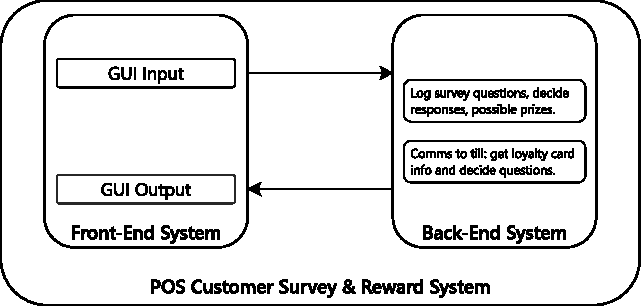
\includegraphics{3_Chapters/4_Chapter_Design/Figures/system_design.pdf}
\caption{Example system level design illustration}
\label{fig:system_design}
\end{figure}

The sections that follow the System Level depends on what your system involves. We have provided an example here of a system that has some Hardware Level aspects, some Software Level aspects and considerations for Integration (in this case setting up a test rig).

\section{Hardware Design}
\label{sec:Design/HardwareDesign}

The Hardware Design sections include significant details on your hardware design, PCB considerations, hardware interfacing and connections and power considerations, among other aspects that are specific to the hardware concerns of your prototype or system being built.  By `significant details' it is suggested that you do not need to go into excessive minutae of the design -- if you are building a significant piece of hardware largely from scratch, then you probably need a good amount of details to explain your choices etc.  You can also use an appendix in which to park information that may be providing extraneous detail that you think is nevertheless needed but is causing the write-up to become too bulky.

\emph{Note:} Even if your project is entirely software, you may still want to have a Hardware section to explain what platform and related components you were using; such information can help others to recreate your experiments, which are a desirable property of a good thesis.  If you are doing software performance tests you would need to provide characteristics of the platform, thus another reason for having a hardware section (but if the hardware section is just there for platform specs, then you can keep the section pretty short, likely not needing more than a page).

It's generally a good idea to include a block diagram and or schematics at this point.  Do not simply have a text-heavy discussion of what parts were used with a detailed schematic and photo of the hardware device that was built (doing so would offload the explanations and logical progression from design to PCB to the examiner to figure out, which is certainly not an advisable approach even if it saves much space).

A representative block diagram, which provides a clear explanation of a specific piece of a design, is presented in Fig.~\ref{fig:POS_Network}.  This figure was drawn in \href{http://www.inkscape.org/}{InkScape}~\cite{InkScape}. When you want to import an InkScape figure (SVG format) into \LaTeX{}, simply save it to PDF (use the drawing extents as the media box area) and include the figure.  This template includes a \texttt{`make figures'} target meant for this purpose.

\begin{figure}[ht]
\centering
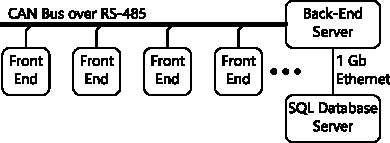
\includegraphics[scale=1.2]{3_Chapters/4_Chapter_Design/Figures/POS_Network.pdf}
\caption{Example hardware level design illustration}
\label{fig:POS_Network}
\end{figure}

\section{Software Design}

The software design section should go from the high-level design aspects, using for example block diagrams or UML class diagrams to explain the main parts of the system, and then going into details of specific operations or algorithms using some or a combination of, for example, pseudocode, UML state charts, UML activity diagrams, flow charts, or other appropriate figures to help the explanations.

You might decide to have some actual code (usually not more than code snippets, i.e., not whole programs) in the Software section, or you might decide to put such details into an implementation section (since the code is something that carries the design into an instantiated implementation).

Things you may have in the Software section include the following:

\begin{itemize}
  \item Software designs drawings (e.g., block diagrams, UML diagrams, etc.)
  \item Algorithms (maybe in pseudocode, or actual code such as MATLAB)
  \item Code snippets (where relevant, used to illustrate how you went from algorithm, or an element of the software design, to executable implemented code)
  \item Implementation and development methods (for example specific software tools that had to be installed, scripts to run, parameters to use; but remember that some of this particular item may be better placed in the methodology -- particularly if it relates to choices that were made earlier on or even before development started.)
\end{itemize}

\section{Implementation}

For a project that is largely hardware based, the implementation section is sometimes rather short, providing photos of the system and explaining some tips and methods on how it was put together (e.g., solutions that were learned for how to solder on parts effectively, or through the implementation experience realising parts that need to be handled with special care etc.) For a project that involves hardware and software, this section could include both tips on getting the hardware together, as well as details about implementing the software.

\section{Integration or Test Rig}

Some research projects require the development of surrounding infrastructure or a suitably conditioned or prepared environment in order to carry out the testing. This may involve developing some sort of test rig into which the prototype is placed or coupled so that testing can be performed on it.  As a simple example, consider a vibration measuring device. If you want to test it in the lab, which has concrete floors but you want to test it for a range of flooring types, it may be necessary to build one or more test rigs that will provide the needed characteristics in order to test the product in a sufficiently authentic situation.

The integration section may alternatively, or in addition to the above point, explain how different subsystems of the system constructed are connected up.  For example, this section might be used to explain the different ways to connect up a system that combines some software on a PC, a complicated DSP platform, and perhaps separate front-end conditioning circuitry, in order to complete experiments to test the achievement of different sub-objectives of the project.

% Chapter 5 - Results

\glsresetall % reset the glossary to expand acronyms again
\chapter[Results]{Results}\label{ch:Results}
\index{Results}

% Results
\section[Results]{Results}
\begin{itemize}
	\item{Describe the experimental setup (ie. Hardware)}
	\item{Describe your experiments}
	\item{Describe your results}
\end{itemize}

This chapter should generally present your finding in the form of figures, tables, equations, code listings, etc. It is for presenting and discussing your findings, which can split into sections if the experiment has multiple parts, or stages.  You might also want to have a `Discussion' or `Discussion of Results' chapter, which may focus on either more detailed discussion of particular results, or more comprehensive discussion of the results and system performance as a whole.  If you have a Discussion of Results section, then you do not want to discuss too much about the specific results in this chapter and rather move the main discussion or reflective considerations of these to the Discussion of Results chapter.

However, and this is an important reminder, ensure that you do have some text of discussion for your results, to take the reader through your results and the figures you may provide.  Make sure not to just put one figure after another without any attempt to explain the sequencing and what is being shown and perhaps some key issues in the figures presented (a monolithic sequence of figure after figure without any attempt at explanation will get undesirable responses from examiners).

If you have an experiments section, it is often useful to have a clear connection of experiment section corresponding to a result section showing results for that test. Examiners often appreciate that sort of clear and consistent structure that is easy to follow.  For example, if you have section~5.1 as Modular Testing, then you could correspond to~6.1 Modular Testing Results (the two sections should be cross-linked with \verb|\label| and \verb|\ref|, in both directions)

\section{Tips for Results Figures}

Include good quality graphs (see Fig.~\ref{fig:r_vs_N_f=0_0005_P=90} for an example).

\begin{figure}[ht]
\centering
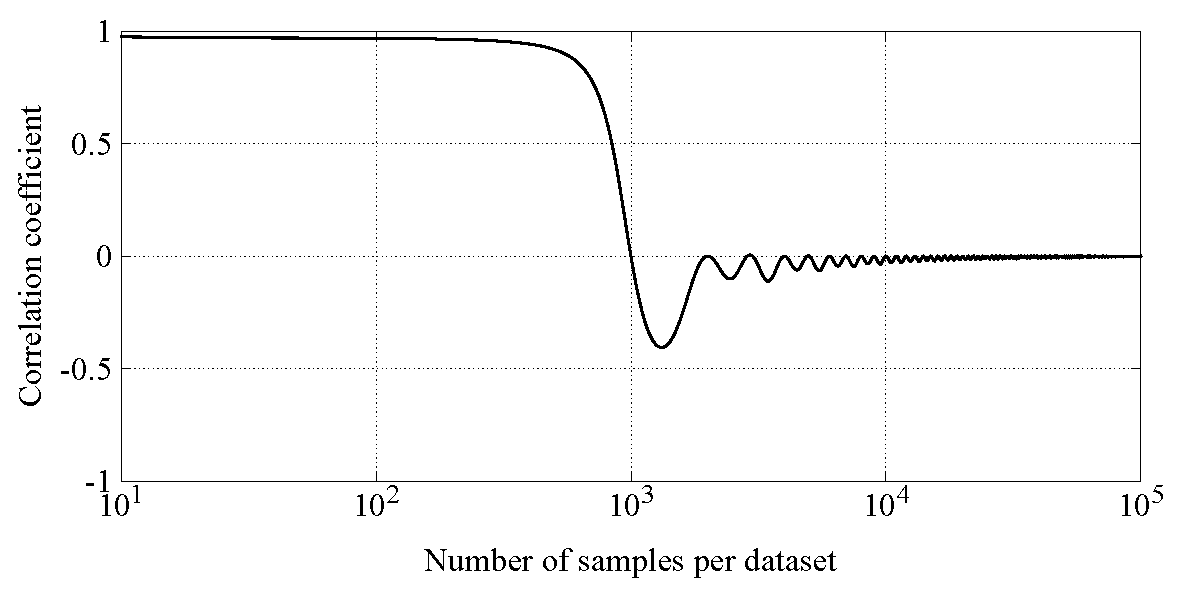
\includegraphics[width=0.8\columnwidth]{3_Chapters/5_Chapter_Results/Figures/r_vs_N_f=0_0005_P=90.pdf}
\caption{The correlation coefficient as a function of sample count}
\label{fig:r_vs_N_f=0_0005_P=90}
\end{figure}

An easy way to obtain more space for an article is to use wide, flat figures, such as Fig.~\ref{fig:Line_Signals}.

\begin{figure}[ht]
\centering
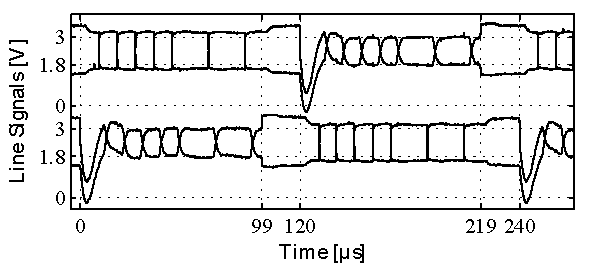
\includegraphics[width=0.8\columnwidth]{3_Chapters/5_Chapter_Results/Figures/Line_Signals.pdf}
\caption{Oscilloscope measurement showing physical line signals on both ends of a transmission line during master switch-over~\cite{Taylor_2016}}
\label{fig:Line_Signals}
\end{figure}


\section{Pictures and screenshots}

When you include screenshots, pdf\LaTeX{} supports JPG and PNG file formats.  PNG is preferred for screenshots, as it is a loss-less format.  JPG is preferred for photos, as it results in a smaller file size.  It's generally a good idea to resize photos (not screenshots) to be no more that 300~dpi, in order to reduce file size. \textbf{Never change the aspect ratio of screenshots and pictures!}

Fig.~\ref{fig:UCT.pdf} shows an example of a PDF image with custom scaling.

\begin{figure}[ht]
\centering

\includegraphics[width=0.35\columnwidth]{3_Chapters/5_Chapter_Results/Figures/UCT.pdf}
\caption{An example image with custom scaling}
\label{fig:UCT.pdf}
\end{figure}

Make sure to always use the best quality image possible.  Use JPEG for photos, PNG for screenshots and PDF (scalable vector graphics) for everything else.  JPEG is lossy, but good for photos, whereas PNG is lossless and good for images with large areas of solid colour.\\

\vspace{5mm}
\hfill
\begin{minipage}[b]{0.3\textwidth}\centering\setlength{\parindent}{0mm}

\includegraphics[width=\textwidth]{3_Chapters/5_Chapter_Results/Figures/UCT.jpg}\\%
{\small (a)~~JPEG}%
\end{minipage}
\hfill
\begin{minipage}[b]{0.3\textwidth}\centering\setlength{\parindent}{0mm}

\includegraphics[width=\textwidth]{3_Chapters/5_Chapter_Results/Figures/UCT.png}\\%
{\small (b)~~PNG}%
\end{minipage}
\hfill
\begin{minipage}[b]{0.3\textwidth}\centering\setlength{\parindent}{0mm}

\includegraphics[width=\textwidth]{3_Chapters/5_Chapter_Results/Figures/UCT.pdf}\\%
{\small (c)~~SVG}%
\end{minipage}
\hfill\mbox{}


% Chapter 6 - Conclusions

\glsresetall % reset the glossary to expand acronyms again
\chapter[Conclusions]{Conclusions}\label{ch:Conclusion}
\index{Conclusions}

% Conclusions
\section{Conclusions}
\begin{itemize}
	\item{Restate the problem. State the novel solution.}
	\item{Summarize what has been accomplished}
	\item{Summarize any limitations}
	\item{What worked really well and has a big impact?}
\end{itemize}

% Future Work
\section{Future Work}
\begin{itemize}
	\item{How do you hope to continue work on this topic?}
	\item{Are there possible extensions?}
	\item{What are some improvements that could be made?}
\end{itemize}

%*******************************************************************************
% 0.8 - BIBLIOGRAPHY
%*******************************************************************************

% Put in \nocite{*} so all entries in the bibliography are included
\nocite{*}

% Print Bibliogrpahy
\phantomsection

% Uncomment for a plain bibliography else use IEEE style below
%\bibliographystyle{plain}
%\bibliography{4_References/References}

% IEEE Bibliography
\bibliographystyle{IEEEtran}
\bibliography{IEEEabrv,4_References/References}

\clearpage

%*******************************************************************************
% 0.9.1 - APPENDICES
%*******************************************************************************

\appendix

% Appendix A
\updatechaptername
\chapter{Supporting Data}

Appendix sections are where you can place large figures, data tables, and spinets of code. Use appendices to your benefit to keep the body of your thesis concise!

The lyrics found below are for your enjoyment, but also serve an important role in demonstrating latex syntax for formatting text and in-text citations.  

\section{Lyrics to Soft Kitty}

\begin{center}
\mbox{}
Soft kitty, warm kitty\\
Little ball of fur\\
Happy kitty, sleepy kitty\\
Purr, purr, purr\\[0.5in]

This has been brought to you by Sheldon Cooper \cite{BigBang}
\end{center}

\clearpage

% Appendix B
\updatechaptername
\chapter{Satirical Support}

This section provides some comic relief. In addition, it serves as an example of how to insert an image into your thesis with proper caption, label and citation.

\begin{figure}[ht]
	\centering
	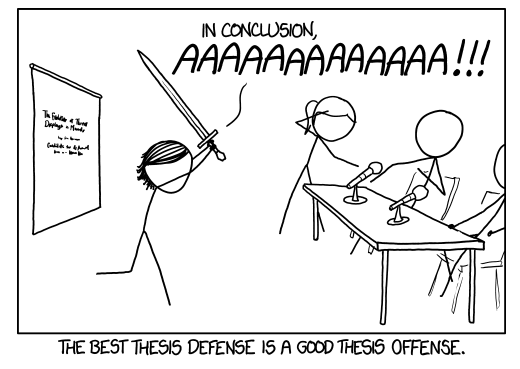
\includegraphics[width = 4.5in]{5_Appendices/Appendix_B/Figures/Thesis_Defence.png}
	\caption{You must prepare to defend your thesis \cite{xkcdThesis}} 
	\label{fig:DEFENCE}
\end{figure}

\clearpage


%*******************************************************************************
% 0.9.2 - INDEX
%*******************************************************************************
% Creates the index
% Uncomment if an INDEX should be created

% \printindex

%*************************************************************************************************************
% 1.0 - END OF DOCUMENT
%*************************************************************************************************************
\end{document}
